\documentclass{article}

\usepackage{amsmath}
\usepackage{fancyvrb} 
\usepackage{floatflt,graphicx}

% Default margins are too wide all the way around.  I reset them here
%\setlength{\topmargin}{-.5in}
%\setlength{\textheight}{9in}
%\setlength{\oddsidemargin}{.125in}
%\setlength{\textwidth}{6.25in}
\begin{document}

\title{A Bayesian Analysis of Global Warming}
\author{Lewis Fishgold}
\date{May 7, 2014}
\maketitle

\section{Introduction}

Global temperature has risen $0.8^\circ$C since the early 20th century \cite{wiki:warming}.
The Intergovernmental Panel on Climate Change ({\sc ipcc}) has stated that
scientists are 90\% certain that the bulk of global warming 
is being caused by human activities including fossil fuel combustion,
cement production, and deforestation.
The geological effects of global warming include the rise of sea level,
changes in patterns of precipitation, and 
expansion of subtropical desert, 
and are expected to have dire consequences for human wellbeing.
The goal of this paper is to perform a Bayesian analysis of the rate
of temperature change in different regions of the world.

\section{Data Set}
I am using the {\sc gistemp} data set 
from {\sc nasa} \cite{hansen2010global}, which contains monthly temperature anomalies for 
the past 100 years for $2^\circ \times 2^\circ$ regions around the globe.
Temperature anomalies measure how much warmer or colder it was in a
particular region and month than the 
average for that region and month, where the average is computed over the period of 1951-1980.

For the sake of simplicity, I am only using data from the past 50 years from 36 regions
lying on a grid over Europe, Asia, Africa, and Australia.
I have also made the data more temporally coarse-grained, by averaging over the months
for each year.
 To get some intuition for what this data is like, Figure~\ref{fig:anomaly} s
 hows the anomaly curve for each of the 36 regions.
Although there is much noise, an upward trend is apparent.

\begin{figure}[h]
\centering
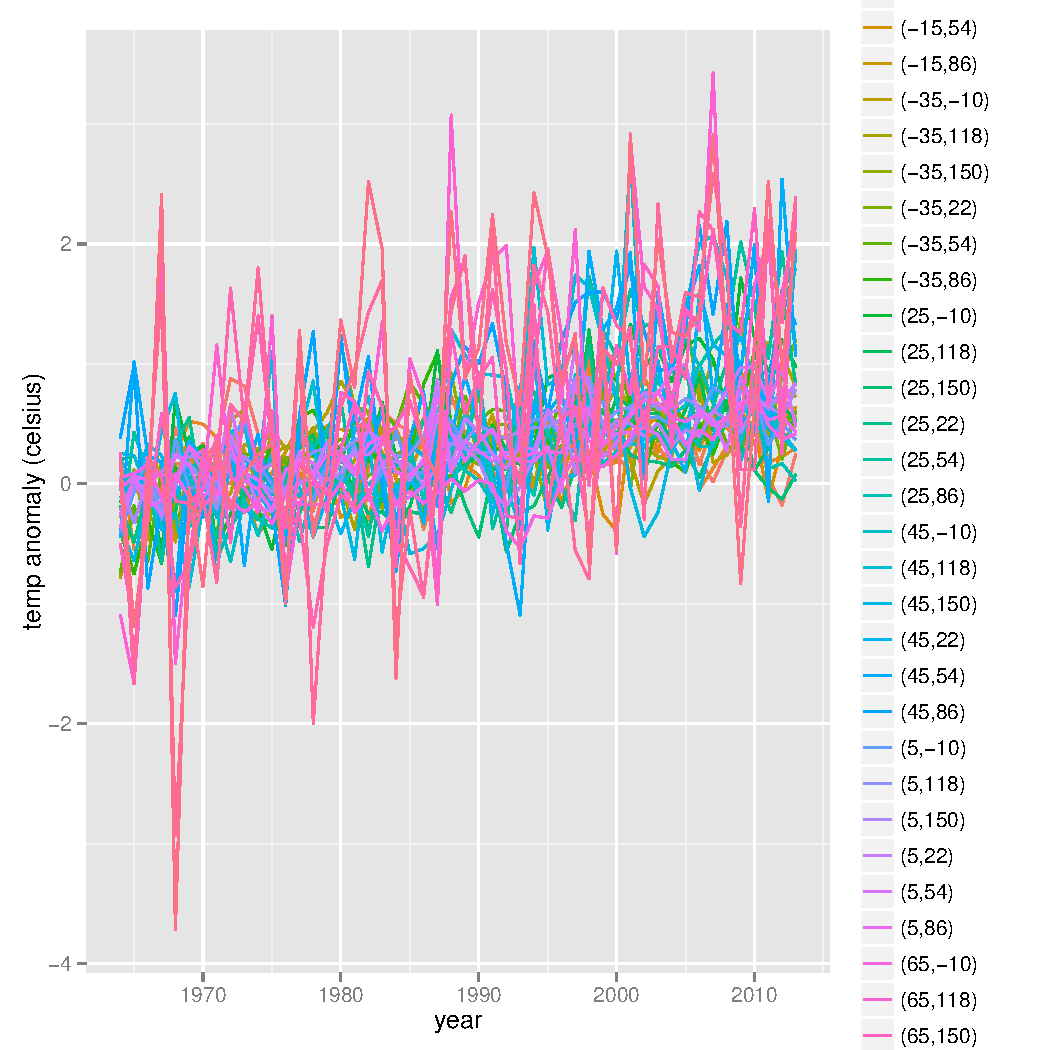
\includegraphics[scale=0.6]{figs/anomaly.pdf}
\caption{The anomaly curve for each of the 36 regions over the past 50 years,
  labelled by latitude and longitude.}
\label{fig:anomaly}
\end{figure}

\section{Models}

To model the data, I used three different linear models.
 Each model attempts to capture the slope in the anomaly curve for each region. 
 The first model, in Figure~\ref{code:pool}, is a linear model with pooling,
 where each region is modelled by the same coefficient.
\begin{figure}[h]
\centering
\VerbatimInput[frame=single,numbers=left,numbersep=6pt]{../code/climate-pool.bug}
\caption{Bugs code for the linear model with pooling.}
\label{code:pool}
\end{figure}
The second model, in Figure~\ref{code:nopool}, is a linear model without
pooling, where each region has its own coefficient.
 I expect that this is a better model than the former, as global warming varies by region.
\begin{figure}[h]
\centering
\VerbatimInput[frame=single,numbers=left,numbersep=6pt]{../code/climate-nopool.bug}
\caption{Bugs code for the linear model without pooling.}
\label{code:nopool}
\end{figure}
The third model, in Figure~\ref{code:hier}, is a hierarchical model where
each region has its own coefficient. 
I expect that this is a better model than the former, as there is a global
process influencing regional temperature change, 
and the hierarchical aspect of the model will help reign in outliers.
\begin{figure}[h]
\centering
\VerbatimInput[frame=single,numbers=left,numbersep=6pt]{../code/climate-hier.bug}
\caption{Bugs code for the hierarchical linear model.}
\label{code:hier}
\end{figure}

In each of the models, the variance parameter for each anomaly curve is shared across regions.
I have centered the data from each region, so that no bias term is necessary in the models.
The prior knowledge I have about global warming is indirectly based on the {\sc gistemp} data
set, 
so using informative priors would amount to using the same data twice.
Therefore, I have used uninformative priors.

\section{Results}
I used a Gibbs sampler to draw 10,000 samples (using 5 chains, 2,000 burnin samples per chain, and no thinning) 
from the posterior distribution for each of the three models.
To assess convergence, I noted that the $\hat{R}$ values from the BRG diagnostic
are close to one for all parameters.
 In addition, the number of effective samples for all parameters is greater than 2000.
 I used DIC (Deviance Information Criterion), an estimate of expected predictive error, to compare models, and the results are in Table~\ref{table:dic}.
 The DIC scores for the non-pooled and hierarchical models are tied, but are better than
 the score of the pooled model.
 I suspect that the hierarchical model did not provide an advantage over the non-pooled
 model because there was enough data to model each slope parameter individually without
 sharing statistical strength between regions.
 
\begin{table}[h]
\centering
\begin{tabular}{ | l | l | }
  \hline
  Model & DIC (lower better) \\ \hline
  Pooled & 2508 \\ \hline
  Not Pooled & 2363 \\ \hline
  Hierarchical & 2364 \\ \hline
\end{tabular}
\caption{}
\label{table:dic}
\end{table}

The following results are based on the hierarchical model.
The 95\% credible intervals for the marginal posteriors of all but one region are above zero, 
indicating that there is warming with a high degree of certainty.
 The 80\% credible intervals are shown in Figure~\ref{fig:hier-posteriors}. 
\begin{figure}[h]
\centering
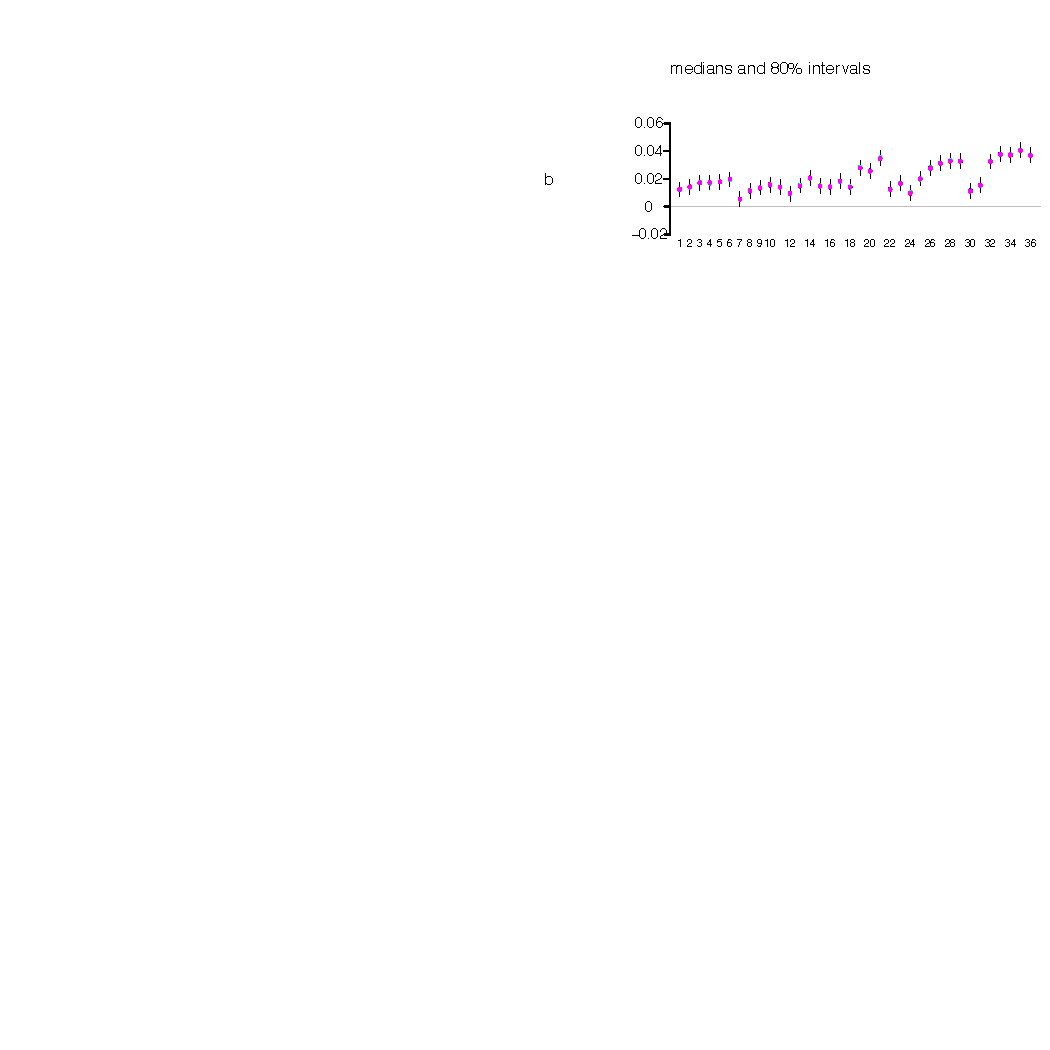
\includegraphics[scale=1.5]{figs/hier-posteriors-cropped.pdf}
\caption{80\% credible intervals for posteriors over hierarchical model.}
\label{fig:hier-posteriors}
\end{figure}
To gain better insight into the variation across regions, 
I have plotted the expected value of the slope for each region on a map
in Figure~\ref{fig:hier-map}.
\begin{figure}[h]
\centering
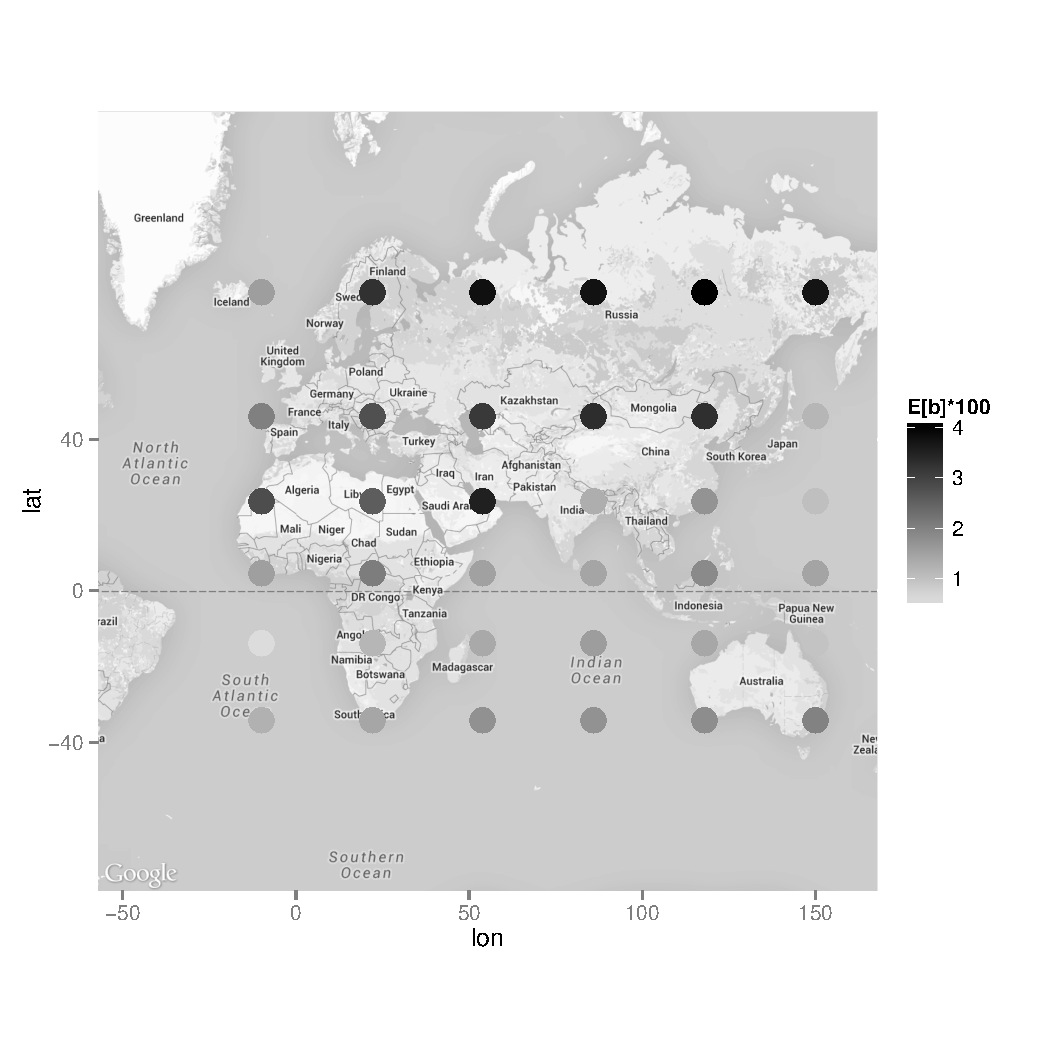
\includegraphics[scale=0.8]{figs/map-hier.pdf}
\caption{The expected rate of change in temperature anomaly per century.}
\label{fig:hier-map}
\end{figure}
 From the plot, it can be seen that the rate varies widely from around $1-4^\circ$ per century, and that 
 global warming tends to be greater at more northern latitudes.

\bibliographystyle{plain}
\bibliography{document.bib}

\end{document}
